\documentclass[12pt]{article}
\usepackage{f1000_styles}
\usepackage[numbers]{natbib}
\usepackage{hyperref}
\hypersetup{colorlinks=false, pdfborderstyle={/S/U/W 1}, pdfborder=0 0 1}
\usepackage{url}
\usepackage{setspace}

\usepackage{booktabs}
\usepackage{doi} % turn DOIs into links

\usepackage{academicons} % for ORCID icon, via https://tex.stackexchange.com/a/534476/212961
\definecolor{idcolor}{HTML}{A6CE39}
\newcommand{\orcid}[1]{\href{https://orcid.org/#1}{\color{idcolor}\aiOrcid}}

\newcommand{\email}[1]{\href{mailto:#1}{#1}}

\usepackage{fontawesome}
\newcommand{\github}[1]{\href{https://github.com/#1}{\faGithub}}
\newcommand{\twitter}[1]{\href{https://twitter.com/#1}{\faTwitter}}

\onehalfspacing

\begin{document}
%\title{CODECHECK: An open-science initiative for the independent execution of computations underlying research articles}
\title{CODECHECK: An Open Science initiative for the independent execution of computations underlying research articles during peer review improves reproducibility}
\author[1,$\ast$]{Daniel~N\"{u}st \orcid{0000-0002-0024-5046} \github{nuest} \twitter{nordholmen}}
\author[2,$\ast$]{Stephen~J~Eglen \orcid{0000-0001-8607-8025} \github{sje30} \twitter{StephenEglen}}
\affil[1]{Institute for Geoinformatics, University of M\"unster, Germany; \email{daniel.nuest@uni-muenster.de}}
\affil[2]{Department of Applied Mathematics and Theoretical Physics, University of Cambridge, GB; \email{sje30@cam.ac.uk}}
\affil[$\ast$]{Contributed equally}
\affil[$$]{Public project for this article is at \url{https://github.com/codecheckers/paper}.}
\maketitle
\begin{abstract}
  In its traditional format, the scientific paper falls short of effectively communicating computational research.
  Since this issue is difficult to address due to lacking incentives, guidance, benefits, recognitions, and reproducibility, we come at this problem from a different angle:
  We propose to introduce, as part of peer review, a system by which the workflows underlying research articles are executed.
  The CODECHECK system, which uses free intrastructure and open tools, relies on five principles and can be integrated into review and publication processes in multiple ways.
  We describe these integrations along multiple dimensions (importance, who, openness, when).
  In collaboration with academic publishers and conferences, we demonstrate CODECHECK with 25 reproductions of diverse scientific publications.
  These CODECHECKs show that asking for reproducible workflows during a collaborative review can effectively improve executability.
  While CODECHECK has clear limitations, it may represent a building block in the Open Science and publishing ecosystems for improving the reproducibility, appreciation, and, potentially, the quality of non-textual research artefacts.
\end{abstract}

\section*{Introduction}\label{introduction}

Many areas of scientific research use computations to either simulate or analyse their data. These computations are becoming increasingly complex and are difficult to explain coherently in a paper \citep{marwick_how_2015}.
To complement the traditional route of sharing research by writing papers,
there is a growing demand to share the underlying artefacts, notably 
code and datasets, so that others can inspect, reproduce or expand that work
(see Figure~\ref{fig:inverse}).
Some of the earliest proponents of this initiative were Buckheit and Donoho \cite{buckheit_wavelab_1995}, who coined what has been called \emph{Claerbout's claim} (extending on \citet{claerbout_electronic_1992}):
\emph{``An article about computational science in a scientific publication 
is \text{not} the scholarship itself, it is merely \textbf{advertising} of
the scholarship. The actual scholarship is the complete software development
environment and the complete set of instructions which generated the 
figures.''}

So, assuming that researchers begin to share more artefacts, how might these artefacts be examined to ensure that they do what they claim?
For example,
most scientific journals now require a data sharing statement that
outlines what data the authors have (or will) share.
Yet, each journal can implement this requirement differently.
At one end of the spectrum, journals have been created to accept ``data papers''
(e.g.,~\href{https://www.nature.com/sdata/}{\emph{Scientific~Data}}, 
\href{https://essd.copernicus.org/}{\emph{Earth System Science Data}}, 
\href{https://rmets.onlinelibrary.wiley.com/journal/20496060}{\emph{Geoscience Data Journal}},
\href{https://bdj.pensoft.net/}{\emph{Biodiversity Data Journal}},
\href{https://openpsychologydata.metajnl.com/}{\emph{Journal of Open Psychology Data}},
\href{https://odjar.org/}{\emph{Open Data Journal for Agricultural Research}},
\href{https://openhealthdata.metajnl.com}{\emph{Journal of Open Health Data}});
these journals have established rigorous procedures by which
the data is validated according to standards in each field.
At the other end of the spectrum, many journals still simply allow authors to state ``Data available upon reasonable request''.
Authors, while possibly well intentioned at the time of writing the article, often cannot provide the data when readers ask for it, as data disappears over time \cite{Vines2014-hf}.

Given that no clear standards yet exist for sharing data, what hope might there be for sharing computer programs?
Both data and software together are required to validate outcomes of a computational analysis, but they differ in that data can be seen as static and inert,
while code requires an environment to be run in and interacted with.
This makes software harder to share.
Our anectodal experiences on this matter suggest that researchers often give a variety of reasons for why code cannot be shared, e.g.,~``there is no documentation'', ``I cannot maintain it'', or ``I do not want to give away my code to competitors''.
Our view, rooted in Open~Science principles\footnote{\url{https://en.wikipedia.org/wiki/Open_science}}, is that sharing code, wherever possible, is good for the community and the individual \cite{Barnes2010-iv,markowetz_five_2015}.
Having code and data openly available and archived provides a valuable resource for others to learn from, even if the code no longer runs or if there is no documentation.
However, with a little effort, we believe that if an independent person can execute an analysis, this is worth documenting as early as possible and that such a focused approach can greatly reduce the barrier to evaluating non-text research materials.
Just as data journals' validations of data and all journals' peer review can provide a ``baseline reassurance'', i.e.,~that a paper has been checked by someone with an understanding of the topic \cite{fyfe_mission_2019}, we think the same baseline should be provided for the workflow underlying a paper.
With this in mind, we have developed a set of principles and an example workflow that provides what we hope is a pragmatic way of checking that a paper's code works.

As this work's main contribution, we offer a thorough description of a process and its variations to integrate a much needed evaluation of computational reproducibility\footnote{Following the Claerbout/Donoho/Peng terminology, see \cite{barba_terminologies_2018}.} into peer review, and we demonstrate its feasibility by means of 25 reproductions across different scientific disciplines.
We call this system CODECHECK as outlined next.

\begin{figure}
% emojis: https://github.com/googlefonts/noto-emoji
% cross mark: u274c
% check mark: u2714
  \centering
  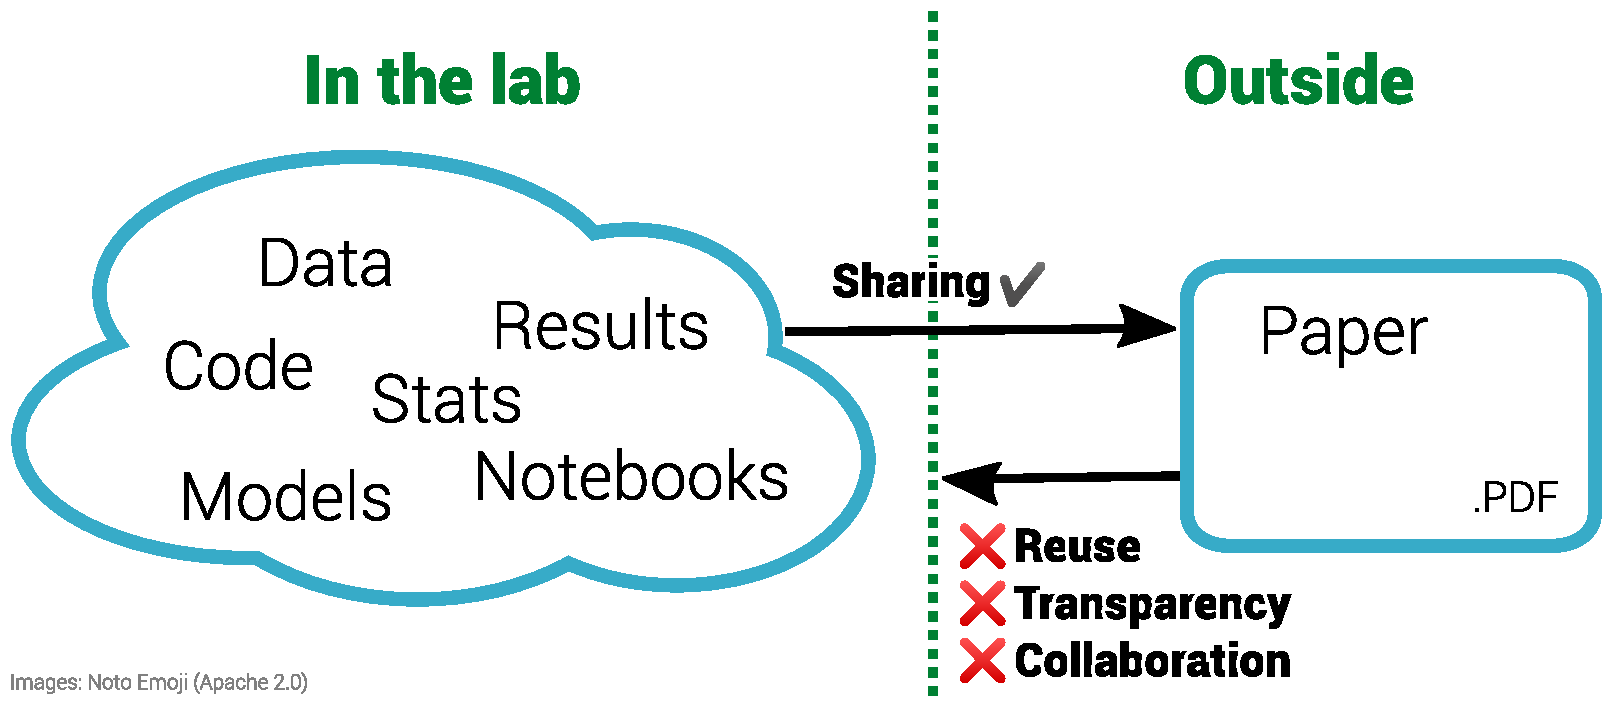
\includegraphics[width=0.7\textwidth]{figs/rr.pdf}
  \caption{The inverse problem in reproducible research. The left
  half of the diagram shows the diverse range of materials used
  within a laboratory. These materials are often then
  condensed for sharing with the outside world via the
  research paper, a static PDF document. Working backwards from the
  PDF to the underlying materials is impossible. This prohibits reuse
  and is not only non-transparent for a specific paper but is also 
  ineffective for science as a whole. By sharing the
  materials on the left, others outside the lab can reproduce
  or build on this work.}
  \label{fig:inverse}
\end{figure}

\section*{What is a CODECHECK?}\label{what-is-a-codecheck}

\subsection*{Workflow and people}\label{workflow-people}

CODECHECK is best demonstrated by way of our example workflow, and later
we expand on the underlying principles. The workflow involves three
groups of people:
(1) the AUTHOR of a paper providing the code to be checked,
(2) the PUBLISHER of a journal interested in publishing the author's paper, and
(3) the CODECHECKER, who checks that the authors's code works.
The workflow we have refined is shown in Figure~\ref{fig:workflow}
and consists of six steps.

\begin{figure}
% original figure source: https://docs.google.com/drawings/d/1tGOZFNZle-oE1Ynw_tLZFmNcv3wgxD0HPs5bXzDOrng/edit
% emojis: https://github.com/googlefonts/noto-emoji and https://github.com/twitter/twemoji
% emoji codes:
% book stack: 1f4da
% package: 1f4e6
% file drawer: 1f5c4
% disk: 1f4be
% document: 1f4c4
% phd: 1f393
% detective: u1f575
% laptop: 1f4bb
% folder: 1f4c1 1f4c2
% receipt: 1f9fe
  \centering
      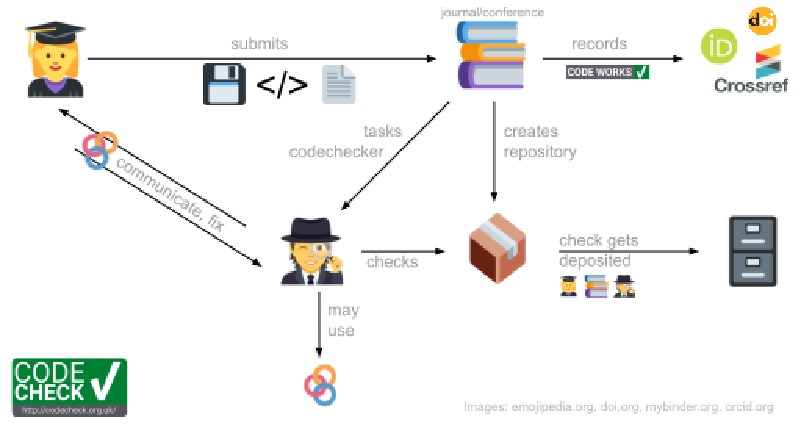
\includegraphics[width=\textwidth]{figs/codecheck_overview.pdf}
  \caption{The CODECHECK example process implementation. Codechecker act as a detectives:
  They investigate and record, but do not fix issues.}
  \label{fig:workflow}
\end{figure}

\textbf{Step 1:} The author submits their manuscript along with the code and data to the PUBLISHER.
The code and data need not be openly available at this point.
However, in many cases the code and data may be published on a code hosting platform,
such as GitHub or GitLab. Ideally, the AUTHOR is expecting the CODECHECK and
prepares for it, e.g.,~by asking a colleague to attempt a reproduction or by 
following the PUBLISHER's guidelines for sharing computational workflows.

\textbf{Step 2:} The publisher finds a CODECHECKER to check the code. This is
analogous to the publisher finding one or more reviewers to evaluate
the paper.
However, a crucial difference is that we suggest the CODECHECKER and the author are able to talk freely and directly to each, regardless how open the scientific peer review process is.

\textbf{Step 3:} The CODECHECKER runs the code, based on instructions provided by
the author. They check if some or all of the results from the paper can be
reproduced. If there are
any problems running the code, the CODECHECKER asks the AUTHOR for help,
updates, or further documentation.
The burden to provide reproducible material lies with the author.
The CODECHECKER then tries to run the code again.
This process iterates until either the CODECHECKER is successful,
or the CODECHECKER concludes the code can not be executed within the context of a CODECHECK.
As part of this process, the CODECHECKER could work entirely locally, relying on their own computing resources, or in the cloud, e.g.,~using the open MyBinder infrastructure \cite{jupyter_binder_2018} or alternatives, some of which are more tailored to scientific publications while others offer commercial options for, e.g.,~publishers (cf. \cite{konkol_publishing_2020}).
A cloud-based infrastructure allows for the CODECHECKER and author to collaboratively improve the code and enforces a complete definition of the computing environment; but, unless secure infrastructure is provided, e.g.,~by the PUBLISHER, this requires the code and data to be published openly online.
Note that the task of the CODECHECKER is to check the ``mechanics'' of the workflow not to evaluate its correctness. 
In the context of mathematics, Stodden et~al. \cite{stodden_setting_2013} distinguish between \emph{verification} and \emph{validation};
following their definition, a CODECHECK ensures verification
\footnote{Note this is a different use from that referred to as the \emph{Verification Reports} article type in the journal \emph{Cortex} \cite{chambers_verification_2020}.},
of computational results, i.e.,~checking that the code correctly produces the output it claims to create, but not a validation, i.e.,~checking that the code implements the right algorithm to solve the specific research problem.
Nevertheless, simply attempting to reproduce an output may highlight a submisison's shortcomings in meeting a journal's requirements (cf.~\cite{christian_journal_2020}) and may effectively increase transparency, thereby improving practices (cf.~\cite{nosek_scientific_2012}) even if the check does not go into every detail.

\textbf{Step 4:} The CODECHECKER writes a certificate stating how the code was
run and includes a copy of outputs (e.g.,~data, figures, or tables) that were
independently generated.
The certificate may include further recommendations to the author on how to improve the material.
The free text in the certificate is the most flexible and feasible way to 
make clear what was really checked, because each workflow is unique.
Since no specific tool or platform should be required, such that no authors are excluded, it would be futile for the CODECHECKER to use automation or fixed checklists.

\textbf{Step 5:} The certificate as well as auxiliary files created
during the check, e.g.,~a specification of a computing environment, data 
subsets or helper scripts, and the original code and data get deposited in
an open archive unless restrictions regarding data size, license or 
sensitivity apply.
Currently, the CODECHECKERs deposit the material on Zenodo themselves, but the PUBLISHER may complete this step after integrating CODECHECK into its review process.
A badge or other visual aid may be added to the deposit and the paper and
link to the certificate.
Although a badge simplifies the CODECHECK into a binary value and risks introducing confusion regarding the extent of the check, especially across disciplines and methods, a badge can provide recognition value and acknowledgement of the completed CODECHECK.
The badge and the actual check are incentives for undertaking the effort needed to provide a readily computationally reproducible workflow.

\textbf{Step 6:} The PUBLISHER can, depending on the timing, provide the
certificate to scientific reviewers or handling editors or publish it
and link between the certificate, the paper, and any repositories 
through metadata. Currently, the CODECHECKER creates these connections on
Zenodo\footnote{
See ``related identifiers'' and ``alternate identifiers'' in the right-hand
sidebar of certificate \texttt{2020-025} \cite{cert-2020-025}.}.
The PUBLISHER also gives credit to the CODECHECKER for their work by depositing
the activity appropriately in scholarly profiles, such as ORCID\footnote{
See peer review contributions in ORCID records at
\url{https://support.orcid.org/hc/en-us/articles/360006971333-Peer-Review}.}.
The PUBLISHER also ensures proper publication metadata, e.g.,~links from the 
certificate repository to the published paper or the original code repository.

\newpage

\subsection*{Variations}\label{variations}

\subsubsection*{Dimensions of CODECHECK workflows}\label{dimensions-of-workflows}

The example workflow leaves room for this process to be implemented differently.
To elaborate on these options, we consider several dimensions in a space of possible CODECHECK workflows, as shown in Figure~\ref{fig:dimensions}, to represent relevant aspects for the involved stakeholders.
These aspects touch on timing, responsibilities, and 
transparency and will be discussed in the following sections.
The options on each dimension have their own pros and cons and can,
for the most part, be freely combined.

\begin{figure}
% original figure source: https://docs.google.com/drawings/d/1q2EdW3Ad-IpcD-CeoR1eIFMJW2fF6OVmDhCtCUmLO1k/edit
  \centering
      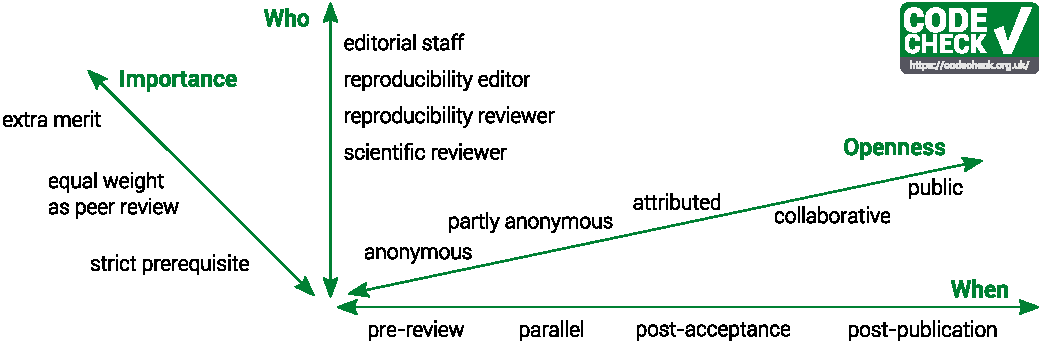
\includegraphics[width=0.8\textwidth]{figs/codecheck_dimensions.pdf}
  \caption{The dimensions of implementing a CODECHECK process.}
  \label{fig:dimensions}
\end{figure}

\subsubsection*{When to do a CODECHECK and with what importance?}
\label{when-to-do-a-codecheck}

The point in time at which a CODECHECK is done and its ascribed importance are closely connected, so we describe the dimensions \emph{When} and \emph{Importance} together.
The earlier a CODECHECK happens in the publishing process, the more it can affect editorial decisions:
Is a paper published, sent back for revisions, or rejected?
Even earlier checks, i.e.,~a CODECHECK of a preprint, may even help to improve the workflow itself, even before a publisher is involved.
As such, codechecking papers could be part of a preprint server's policy or simply be initiated by interested readers and community members.

Publishers could introduce a CODECHECK as a \textbf{strict prerequisite}.
As this can reduce the workload of reviewers, such a check should not occur late in the review process.
Yet, the later in the review process the check happens, the easier is it to allow bidirectional communication between the author and codechecker, e.g., because the author might already be notified of the paper's acceptance and may more freely share materials online closer to the paper's publication date.
A \textbf{pre-review} CODECHECK would allow editors to only send a submission out for peer review if it passes the check, or to include the certificate in the submission package provided to the reviewers.
Reviewers may then judge the the relevance of the computations for the results of the work, or follow journal guidelines regarding how strictly to apply the check's outcomes in their evaluation.

A CODECHECK may also be conducted in \textbf{parallel} to the scientific peer review.
This puts less burden on the turnaround time for the check, yet it only makes the outcomes available during the final consideration by the handling editor.
The check could also be assigned after suggestion by a reviewer, which would remove the need for submissions to undergo a pre-review screening.
However, soliciting such a ``specialist review'' is much less desirable than having a regular CODECHECK, thus avoiding the situation in which some submissions get special treatment.
In both cases, a CODECHECK could then be awarded \textbf{equal weight} compared to the other reviews for the editor's decision.

A \textbf{post-acceptance} CODECHECK would have the smallest impact on editorial decisions and may simply provide \textbf{extra merit} on top of the submission's acceptance.
This is the least impactful solution in which all material is still evaluated and the results of the check are properly acknowledged, because the check can be completed before the publication of the paper.
The GIScience group of checks (see below) falls into this category:
By displaying a badge on the volume and article landing pages, the AGILE conference highlights articles whose reproducibility was successfully reviewed.
Similarly, in collaborations with journals, some GIScience have been checked while the authors worked on revisions.

A CODECHECK may also be conducted \textbf{post-publication}, though it would require someone to update the article and article metadata to reference the check; otherwise, readers would presumably not be aware of it.
In general, publishers hesite to make such revisions to published articles.
While this option has the least impact on current publishing practices and enables open discourse, it also has the smallest effect on the original submission and does not acknowledge the importance of reproducible workflows for ensuring good scientific practice.

In general, the timing of a CODECHECK needs to be connected with 
established or typical scholarly communication process.
While more radical ideas do exist for changing the paradigms of how researchers can more granually share their work much
\footnote{For example Octopus, \url{https://science-octopus.org/about}, or Hypergraph, \url{https://www.libscie.org/hypergraph}.},
% mimosa is another platform idea, but no real prototype AFAICT:
% https://projects.invisionapp.com/share/E9Z3RKE7W3P#/screens/436978924
% https://docs.google.com/presentation/d/1V_K8hghgnvGfEtW7TdwtowTveZyy4Qs8rMemNyHx_Dg/edit#slide=id.p
an evolutionary approach has value, and we do not yet suggest to completely eliminating research papers as a way of sharing work.
Enhancing existing processes with CODECHECKs allows communities to transition towards more open practices at their own pace and ensure that no one is unfaily left behind.
When integrating a CODECHECK into existing review and publication processes, the \emph{turnaround time} is crucial.
Depending on when and who conducts the check, it might be done quickly or it might add considerable time to how long it takes from submission to publication.
In our first checks, we found that a CODECHECK generally takes from 2-5 hours, with some outliers on the higher end.
This time includes writing and publishing the certificate but excludes the time for actual computations.
These efforts are comparable to the time needed to peer review a submission,
which aligns with the efforts some volunteer codecheckers are willing to
make.
However, the time includes a considerable amount of communicating about the
process, especially regarding who publishes which document when, so that proper
cross-referencing between paper and certificate is ensured via persistent
identifiers.
When integrated into a peer review platform, this handling of documents should
become much more effective and reduce organisational overhead.

\subsubsection*{Openness, or ``Who knows who?''}\label{who-knows-who}

The topic of anonymity is broadly discussed, especially in the push towards
open peer review as part of the Open Science movement 
(cf. \cite{ross-hellauer_guidelines_2019}).
Without taking a strong stance on this topic, the general motivation 
behind CODECHECK
for higher transparency and reproducibility does indeed favour a more open 
review process.
However, anonymity can also serve to protect individuals \cite{tennant_limitations_2020}, e.g.,~junior scientists, whereas revealing of names from tenured researchers might be more reasonable to require.
The possible negative effects of a non-anonymous review are reduced if a CODECHECK is not relevant for a journal's decision to accept or reject, but that is, of course, not desirable when the goal is higher transparency and reproducibility.
Instead, we argue that a CODECHECK is technical process that should in general find fixable problems; it is not aimed at giving an opinion or identifying a faulty approach.
It is technically possible for a nonsense workflow to receive
a CODECHECK certificate.
If passing a CODECHECK becomes mandatory, the full transparency may have to be 
revisited as the relations between authors and codecheckers would fall under the
same social and community challenges as non-anonymous peer review
(cf.~\cite{everythinghertz123}).
% previous sentenc inspired by https://osf.io/9cftx/

The technical nature of the check and the challenge of providing sufficient documentation is why we see great benefits in allowing for bidirectional communication between author and codechecker.
Instead of trying to
fix problems or guess the next step, the codechecker can ask the author to 
rework the documentation or the update code.
Instead of struggling to provide perfect instructions and as a result possibly not sharing any code or data, the author can make a best effort to document sufficiently.
Of course, the codechecker may also provide a fix within the code instead
of lengthily describing a small change if it can be quickly done.
Authors and readers can profit from a codecheckers' experience and approach, as during the check they may create useful and instructive files, e.g.,~a machine-readable computing environment specification.
While communication between author and codechecker may be facilitated in an 
anonymous way by the 
publisher, it most likely only helps to protect the identity of the codechecker, because, especially when codebases are of a certain size, not trivial, or if very specialised, they are almost impossible to fully anonymise.
Therefore, the most effective and desirable situation for the stakeholders is to hold a non-anonymous and collaborative CODECHECK.
The contributions by the codechecker may even be integrated into
the code of the workflow and be acknowledged as code commits. This way, 
proper credit can be given within the research software development community.
Nevertheless, depending on the needs represented by other dimensions,
the aspect of ``Who knows who?'' may be the most flexible.

\subsubsection*{Who does the CODECHECK?}\label{who-does-the-codecheck}

The options for who can conduct a CODECHECK require a somewhat complex matching of a combination of skills and availability.
Ideally, thecodechecker has a matching code \emph{and} domain expertise; for example, to check a workflow based on Python code analysing neuroimaging datasets, the codechecker should ideally be experienced in Python and neuroimaging analysis.
However,
a well-documented workflow should be executable by any person with a basic
understanding of computers. Naturally, the more prerequisite knowledge the
codechecker has, the less time is needed to understand the goals and 
the mechanics of an analysis.
From our experiences, the priority should be given to matching technical expertise first, as lacking knowledge in setting up a computing environment with a particular language or tool is much more of a problem than assessing the outcome, e.g.,~comparing created figures with the original, without an in-depth understanding of the science.
The depth of the check will mostly be driven by the time required and expertise of the checker, though in general, we expect a CODECHECK not to evaluate performance (e.g.,~it will not check whether a racing car has the best apex speed) but to assess operation free of failure (i.e.,~is it a car with 4 wheels and does it move forwards when accelerating).
This depth can be seen independent of the check's importance, as long as it is communicated clearly to all stakeholders, most importantly authors and readers.

The concrete people to provide such expertise can range from researchers,
possibly drawn from the regular pool of volunteer
\textbf{scientific reviewers}, or from a special group of
\textbf{reproducibility reviewers} via specific roles
such as \textbf{reproducibility editors}, to experts working as part of
\textbf{editorial staff} with a publisher. If the regular reviewers
are relied upon, the editor's task to find suitable ones becomes more
tedious; extra information such as software familiarity would have to be
modelled in review platforms.

We consider a \emph{single codechecker} to be enough, unlike peer review where
multiple referees are common.
Because of the technical focus, determining whether the concrete outputs produced by the author and the codechecker, who can collaborate to solve any issues, actually match should be a very factual process and not require much debate or opinion.
Code usually harbours systematic and repeatable mistakes and is thereby more reliable and auditable than processes controlled by humans \cite{tibav:42484}, e.g.,~in a laboratory.
Depending on the importance of the CODECHECK
(see above), a mediator, e.g.,~the editor, or a
second opinion might be warranted in rare cases.

We also see a great opportunity to involve \emph{early-career researchers} (ECRs) as codecheckers.
ECRs arguably have a high interest in learning
about the latest tools and technologies, as they are building up their own
expertise and specialisation.
CODECHECK offes a way for ECRs to gain insights into the latest science and at the same time can help increase the appreciation of reproduction efforts, a combination that is of particular interest.
\emph{ReScience X}, a journal devoted to reproduction and replication experiments \cite{roesch_new_2020}, shares an interest in this combination.
Further, ECRs are often much more familiar with latest technology and tend to be early adopters, thus also making them likely to author CODECHECK-ready manuscripts
\footnote{Cf. the 77\% of 141 registered reports that were submitted to leading Neuroscience journals by ECRs \cite{chambers_registered_2019}.}.
As ECRs are introduced to peer review as codecheckers, they may transition into the role of scientific reviewer over time.
Another potential highlight is that during the codechecking process, a senior codechecker may support a junior codechecker, which would be the opposite of what happens during general peer review, which is largely an unsupervised process, i.e.,~rarely are reviewers taught how to do it.
Overall, we see several opportunities and benefits to setting up a new process for CODECHECKING with a clear commitment to openness and transparency, independent of the current peer review process (see \emph{Openness} dimension).

Having the codechecker be part of the publisher's \textbf{editorial staff} represents the most controlled but also
resource-intensive option.
Hiring the required technical and or domain expertise will put a financial burden on the publisher, of course, but such a commitment would also show that publishers are investing in reproducibility.
Codecheckers on staff would positively impact the submission experience and the external perception, because having an in-house codechecker would make the process easier to control and would ensure the author gets an external, unbiased review.
Furthermore, a staff codechecker would also reduce the challenges regarding open communication and awarding credit, as in-house personnel may more readily be given access to submission material would receive a salary instead of public credit as part of the scientific community.
Yet, keeping diverse specialists on as staff to realise a codechecking process is 
unlikely to be feasible for small or independent publishers.

In contrast, for researchers it can be very important to be publicly credited
for their activity as a reviewer.
A regular
review may be listed in public databases (e.g.,~ORCID
\footnote{\href{https://support.orcid.org/hc/en-us/articles/360006971333-Peer-Review}{https://support.orcid.org/hc/en-us/articles/360006971333-Peer-Review}} or commercial offerings such as Publons
\footnote{\href{https://publons.com/}{https://publons.com/}} or 
ReviewerCredits\footnote{\href{https://www.reviewercredits.com/}{https://www.reviewercredits.com/}});
a codechecker should be similarly listed.
The number of scientific reviews is of course only a coarse indicator of an individual's community contribution, yet it is unclear if a regular reviewer, who conductsa regular scientific review and in addition also conducts a CODECHECK, should be credited twice.
In this case, the published CODECHECK certificate and possibly the published peer review can clearly describe the possibly large efforts put into both.

The codechecker community\footnote{\href{https://github.com/codecheckers/codecheckers/}{https://github.com/codecheckers/codecheckers/}}
currently has over 20 individuals who signed up in the last 12 months as volunteer codecheckers after talks given on the project, even though no checks are actively being requested in collaboration with journals.
These volunteer's motivations, mentioned in the registration information\footnote{\url{https://github.com/codecheckers/codecheckers/labels/registration}}, are that they want to
support reproducible research and Open Science,
establish a culture of open and reproducible science,
be part of making this culture the norm,
improve coding skills,
give back to the community,
gain experience in helping scientists with their code,
reduce the amount of bad scientific code, 
encourage a culture that reduces friction in sharing or passing along on academic codebases,
learn from other people's mistakes;
many are also motivated simply by curiosity.
We see benefits to an open shared list of codecheckers across journals rather than a private in-house group, as this may allow for better matches regarding expertise and more even sharing of the workload.
Overall, this community will aim to ensure that CODECHECK is a viable option not just for large publishers, independent of their financial model, but also for independent no-cost Open Access journals.

\section*{Core principles}\label{core-principles}

The example workflow and variations outlined above reflect our current
views on how a workflow execution and code checking should be performed as part of peer review.
They are not set in stone, but we do believe the following core principles underpin our CODECHECK process:

\textbf{1. Codecheckers record but don't investigate or fix.} \\
The codechecker follows the instructions provided by the author in running
the code. If any steps are unclear, or if code does not run correctly,
the codechecker records this fact and then communicates this
information to the author. We believe that the job of the codechecker is
not to fix all these problems but simply to report them and await a
fix from the author.
The level of documentation that is needed for third parties
to reproduce a workflow is extremely hard to get right, and too often this 
uncertainty leads researchers to give up and not document it at all.
The conversation with a codechecker fixes this problem.

\textbf{2. Communication between humans is key.} \\ 
Some code may
work without any interaction (e.g., CODECHECK certificate \texttt{2020-013}
\cite{cert-2020-013}) but more often there are hidden
dependencies that need to be found or software installations that need to be adjusted for a particular system.
Allowing the (human) codechecker to communicate
directly and openly with each other should make this process as
constructive as possible. We feel that routing this conversation
(possibly anonymously) through a publisher would slow things down and
reduce the chances for community building as well as obscure some of the lessons
learned for both authors and codecheckers.

\textbf{3. Credit is given to codecheckers.} \\ 
The value of performing a
CODECHECK is comparable to that of a scientific peer review, and
it may also require a similar amount of time. Therefore,
the codechecker's activity should be publicly recorded and mentioned in the
published paper.
The public record can be realised by publishing the certificate in a 
citable form (i.e.,~with a DOI, as conducted in the community CODECHECK
process), by listing codecheckers on the journal's website or, ideally, by
publishing the checks alongside peer review activities in public databases.

\textbf{4. Workflows must be auditable.} \\ 
This requires that the codechecker 
has at least enough material to validate the workflow outputs submitted by 
the authors. Stark~\cite{stark_before_2018} calls this ``preproducibility''
and the ICERM report \cite{stodden_setting_2013} defines the level
``Auditable Research'' similarly.
Every community may establish their own good practices or adapt generic
concepts and practical tools, such as publishing all building blocks
of science in a research compendium
\footnote{\url{https://research-compendium.science/}}.
A completed check means that code could be executed at least once without
critical errors or
warnings using the provided instructions, and, therefore, all code and data 
was given and could be investigated more deeply or extended in the future.
Ideally, this is a ``one~click'' step, but achieving this requires particular 
skills and a sufficient level of documentation for 
third parties. Furthermore, automation may lead to people gaming the system
or reliance on technology, which can often hide important details.
All such aspects can reduce the understandability of the material, so we estimate our approach to codechecking, done without automation and with open human communication, to be the best way to ensure long-term transparency and usefulness.
We acknowledge that others have argued in favour of bitwise reproducibility
because, in the long run, it can be automated\footnote{Konrad Hinsen on 
Twitter: \url{https://twitter.com/khinsen/status/1242842759733665799}},
but until then we need CODECHECK's approach.

\textbf{5. Open by default and transitional by disposition.} \\ 
By default, unless there are strong
reasons to the contrary (e.g.,~sensitive data on human subjects), all code and
data, both from author and codechecker, will be made freely available, 
i.e.,~under open licenses, before or when the certificate is published.
Note that openness is not required for the paper itself, as to accommodate 
journals in their transition to sustainable Open Access models.
The code and data publication should follow community good practices.
By disposition, a CODECHECK workflow should be designed (a) with a recognition of
shortcomings in asserting reproducibility of submissions and (b)
with an understanding of the
complex situation that led to this. However, establishing a CODECHECK workflow
should go hand in hand with initiatives aiming to improve education
around reproducibility of methods and communication surrounding comprehensive 
computational workflows.
The long term goal is for a specific community or
journal's target audience to reach a state where the level of verification 
ensured by codecheckers becomes part of peer review and a regular
merit of all accepted papers.

\section*{Implementation}\label{implementation}

\subsection*{Register}\label{register}

We have a curated list of 25 certificates available at
\url{https://codecheck.org.uk/register}.
Table~\ref{tab:register} lists the certificates completed to date
along with citations to the original papers.
These CODECHECKs fall into three themes:
(1) classic and current papers from computational neuroscience,
(2) COVID-19 modelling preprints, and
(3) GIScience.

The first theme was the initial set of papers used to explore the concept
of CODECHECK. 
The idea was to take very well known historical articles from a 
specific domain, in this case the work area of SJE, possibly 
as as a conversation starter for potential collaborating journals.
This intention was brought to the first CODECHECK (certificate number
\texttt{2020-001}) performed before publication on an article for the journal
\emph{GigaScience}, which successfully reproduced the visualisations,
though not the full machine learning process.

The second theme is rather opportunistic. As the COVID-19 pandemic swept
over the globe, we hoped to contribute a small part to science's answer
to the unknown virus. The checks were solicited through community interaction
%Several COVID-19 models have been done during the time of peer review of these papers,
or by our initiative rather than requested from journals, but some certificates
have since then been acknowledged in reviewed papers
\cite{Davies2020-vj,kucharski_effectiveness_2020}. Unlike many claims in
popular media at the time,
% reference missing here TODO SJE, you had a note about some Noorden news piece
we found the results of Report 9, a model of the UK lockdown procedures,
to be reproducible (certificate number \texttt{2020-10}).

The third theme represents DN's service as a Reproducibility Reviewer at the AGILE conference series, where the \emph{Reproducible AGILE} Initiative \cite{reproducible_agile} established a process for reproducing workflows at the AGILE conference series independent of CODECHECK \cite{nust_improving_2020}.
While using slightly different terms and infrastructure (``reproducibility
reports'' are published on the Open Science Framework (OSF) instead of certificates on Zenodo) the 
AGILE reproducibility reviews adhere to the CODECHECK principles.
Furthermore, a small number of checks were completed as part of peer reviews
for GIScience journals.

\begin{table}
  \footnotesize

  \centering

  \begin{tabular}{llp{12cm}}
    \toprule
    \textbf{Certificate} & \textbf{Research area} & \textbf{Description} \\ \midrule
    \texttt{2020-001} \cite{cert-2020-001} & Machine learning & Code for benchmarking ML classification tool checked post acceptance of manuscript and before its publication in \textit{Gigascience} \cite{Piccolo2020-lo}. \\
    \texttt{2020-002}  \cite{cert-2020-002} & Neuroscience & Code written for this project checked by second project member as demonstration using paper from 1997 showing unsupervised learning from natural images \cite{Hancock1992-mp}. \\
    \texttt{2020-003}  \cite{cert-2020-003} & Neuroscience &  Code written for this project checked by second project member as demonstration using classic paper on models of associative memory \cite{Hopfield1982-mz}. \\
    \texttt{2020-004}  \cite{cert-2020-004} & Neuroscience & Code written for this project checked by second project member as demonstration using classic paper on cart-pole balancing problem \cite{Barto1983-rg}. \\
    \texttt{2020-005}  \cite{cert-2020-005} & Neuroscience & Check of independent reimplementation of spike-timing-dependent plasticity (STDP) model \cite{larisch_re_2019} conducted as demonstration for this paper. \\ % Python ANNarchy
    \texttt{2020-006}  \cite{cert-2020-006} & Neuroscience & Check of independent reimplementation of a generalized linear integrate-and-fire neural model \cite{detorakis_re_2017} conducted as demonstration for this paper. \\
    \texttt{2020-007}  \cite{cert-2020-007} & Neuroscience & Check of independent reimplementation of analysing spike patterns of neurons \cite{hathway_re_2018} conducted as demonstration for this paper. \\
    \texttt{2020-008}  \cite{cert-2020-008} & COVID-19 & Code for modelling of interventions on COVID-19 cases in the UK checked at preprint stage \cite{davies-preprint-2020} and later published \cite{Davies2020-vj}. \\
    \texttt{2020-009}  \cite{cert-2020-009} & COVID-19 & Code for analysis of effectiveness of measures to reduce transmission of SARS-CoV-2 checked as preprint \cite{kucharski-preprint-2020} and later published \cite{kucharski_effectiveness_2020}. \\ % R, check mentiond in acks, but not linked
    \texttt{2020-010}  \cite{cert-2020-010} & COVID-19 & Code for analysis of non-pharmaceutical interventions (Report 9) checked as a preprint \cite{ferguson_report_2020}. \\ % CovidSim
    \texttt{2020-011}  \cite{cert-2020-011} & COVID-19 & Code for modelling of COVID-19 spread across Europe was provided by authors and checked while paper was in press \cite{flaxman_estimating_2020}. \\
    \texttt{2020-012}  \cite{cert-2020-012} & COVID-19 & Code for modelling of COVID-19 spread across the USA was checked as preprint \cite{unwin_report_2020} and later published \cite{unwin_state-level_2020}. \\
    \texttt{2020-013}  \cite{cert-2020-013} & Neuroscience & Code for analsis of rest-activity patterns in people wihout con-mediated vision was checked as a preprint \cite{Spitschan2020.06.02.129502} after direct contact with the authors. \\ % MATLAB
    \texttt{2020-014}  \cite{cert-2020-014} & Neuroscience & Code for analysis of pertubation patterns of neural activity was checked after publication as part of publisher collaboration \cite{Sadeh2020}. \\ % MATLAB
    \texttt{2020-015}  \cite{cert-2020-015} & Neuroscience & Code for a neural network model for human focal seizures was checked after publication as part of publisher collaboration \cite{Liou2020}. \\ % MATLAB
    \texttt{2020-016}  \cite{cert-2020-016} & GIScience & Code for models demonstrating the Modifiable Aral Unit Problem (MAUP) in spatial data science \cite{Brunsdon2020} was checked during peer review. \\ % R
    \texttt{2020-017}  \cite{cert-2020-017} & GIScience & Code for spatial data handling, analysis, and visualisation using a variety of R packages \cite{Bivand2020} was checked after peer review before publication. \\ % R
    \texttt{2020-018}  \cite{cert-2020-018} & GIScience & AGILE conference reproducibility report using a demonstration data subset with cellular automaton for modeling dynamic phenomena \cite{Hojati2020}. \\ % R
    \texttt{2020-019}  \cite{cert-2020-019} & GIScience & AGILE conference reproducibility report with subsampled dataset for reachability analysis of suburban transportation using shared cars \cite{Illium2020}. \\
    \texttt{2020-020}  \cite{cert-2020-020} & GIScience & AGILE conference reproducibility report using a container for checking in-database windows operators for processing spatio-temporal data \cite{Werner2020}. \\ % Python + PostGIS
    \texttt{2020-021}  \cite{cert-2020-021} & GIScience & AGILE conference reproducibility report checking code for comparing supervised machine learning models for spatial nominal entity recognition \cite{Medad2020}. \\ % Python
    \texttt{2020-022}  \cite{cert-2020-022} & GIScience & AGILE conference reproducibility report checking code for visualising text analysis on intents and concepts from geo-analytic questions \cite{Xu2020}. \\ % Python
    \texttt{2020-023}  \cite{cert-2020-023} & GIScience & AGILE conference reproducibility report on analysis of spatial footprints of geo-tagged extreme weather events from social media \cite{Owuor2020}. \\
    \texttt{2020-024}  \cite{cert-2020-024} & Neuroscience & Code for multi-agent system for concept drift detection in electromyography \cite{vieira_driftage_2020} was checked during peer review. \\ % R
    \texttt{2020-025}  \cite{cert-2020-025} & GIScience & Adaptation and application of Local Indicators for Categorical Data (LICD) to archaeological data \cite{carrer_application_2021} was checked after peer review before publication. \\ % R
    \\ \bottomrule
  \end{tabular}
  \caption{Register of completed certificates as of December 2020. An interactive version
  is available at \url{http://codecheck.org.uk/register}.
  }
  \label{tab:register}
\end{table}

\subsection*{Annotated certificate and check metadata}\label{annotated-certificate}

At the completion of each CODECHECK, the codechecker writes a certificate stating which outputs from the original article, i.e.,~numbers, figures or tables, could be reproduced.
This certificate is made openly
available so that all readers of the article can see which elements
were reproduced and what limitations or issues were faced.
The certificate also includes links to the code
and data used by the codechecker, allowing others to build on the
work.
The format of the certificates has evolved slightly during the
project, as we have learnt to automate different aspects of the
certification, such as inserting figures into certificate documents
and managing core metadata surrounding a check.
The metadata is stored in a machine-readable structured file in YAML,
the CODECHECK configuration file \texttt{codecheck.yml}\footnote{
See technical specification of the CODECHECK configuration file at
\url{https://codecheck.org.uk/spec/config/latest/}.}.
The configuration file enables current and future automation of workflows and
meta-analyses.

To demonstrate the typical contents of a certificate and the underlying
metadata, 
Figure~\ref{fig:cert} shows the first four out of ten
pages of the certificate \texttt{2020-012} \cite{cert-2020-012} with
annotations.
The referenced article \cite{unwin_report_2020} describes the modelling of COVID-19 across the USA.
Figure~\ref{fig:cert}A shows the certificate number and its DOI,
which points to the certificate and any supplemental files on Zenodo.
The CODECHECK logo is
added for recognition and to denote successful reproduction.
Figure~\ref{fig:cert}B provides the key metadata as a table generated
from the \texttt{codecheck.yml}; in particular it names the paper that
was checked (title, DOI), the authors, the codechecker, when the check was performed,
and in which repository related material is
accessible.
Figure~\ref{fig:cert}C shows a textual summary of how the CODECHECK was
performed and any interesting findings.
Figure~\ref{fig:cert}D (page 2 of the certificate) shows a table that
lists the outputs that were generated from the check based on the 
manifest of output files in the CODECHECK.
The certificate's file table shows the file name, the description stating to
which figure/table each file should be compared in the original paper, and
the size of the file.
Page 3 of the certificate,
as Figure~\ref{fig:cert}E shows, provides detailed notes from the
codechecker. In this particular example, the notes document what steps were 
needed to initialize the environment and run the code and that the execution
took quite long to run -- about 17~hours. Finally, on page 4 of
the certificate, we see the first output that was generated by the
CODECHECK (Figure~\ref{fig:cert}F). In this case, the figure matches
figure~4 of \cite{unwin_report_2020}.
Subsequent pages of the certificate show other outputs and the computing
environment in which the certificate itself was created (not shown here).

\begin{figure}
  \centering
  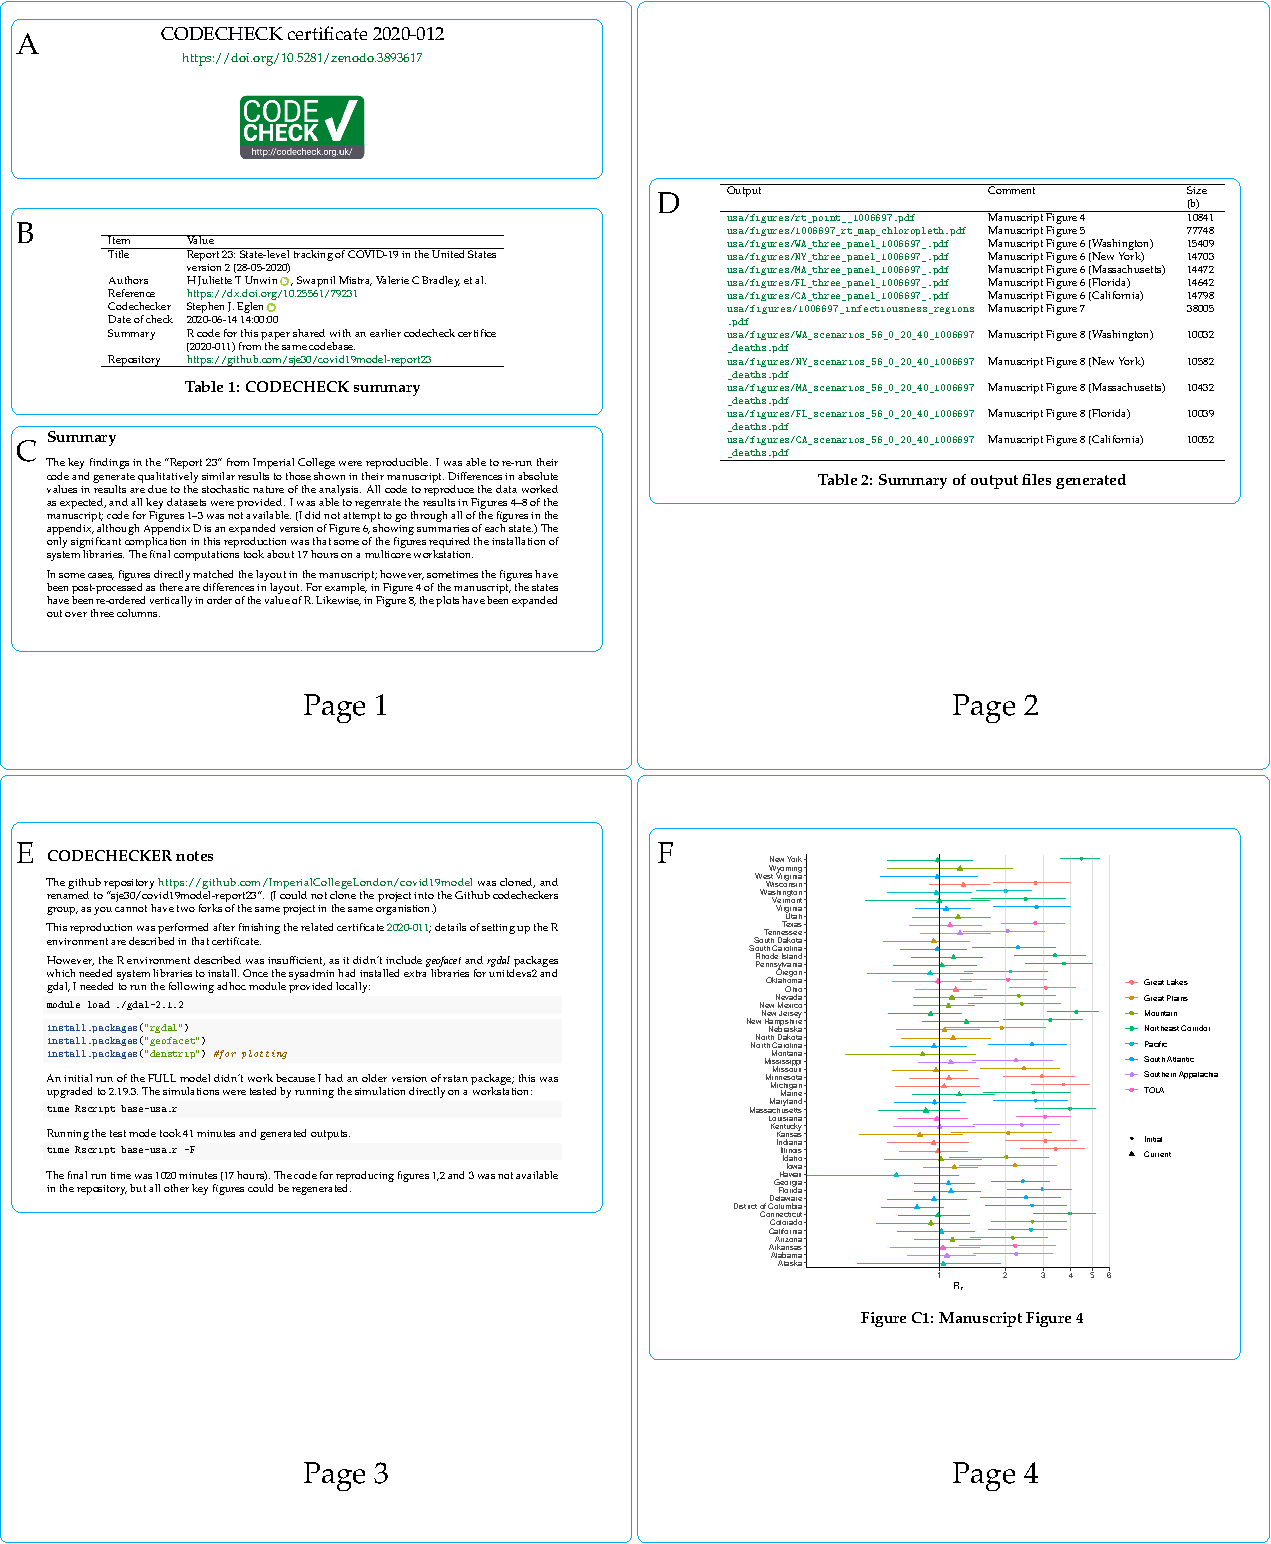
\includegraphics[width=\textwidth]{figs/annotate-cert-crop.pdf}
  \caption{Annotated certificate \texttt{2020-012} \cite{cert-2020-012} (first four pages only).}
  \label{fig:cert}
\end{figure}

\subsection*{Tools and resources}\label{tools}

To run the system, we rely on freely available infrastructure, more 
specifically GitHub and Zenodo.
The \texttt{codecheckers} \textbf{GitHub} organisation\footnote{
\url{https://github.com/codecheckers}} contains projects for managing the
project website, the community of codecheckers, community discussions,
forks of checked code repositories, and the main register of 
CODECHECKs. Both the website\footnote{
\url{https://codecheck.org.uk/}} and the register\footnote{
\url{https://codecheck.org.uk/register}} are hosted as GitHub
pages. The register is a single table in CSV format that
connects the certificate identifier with the repository associated with
a specific conducted CODECHECK. Each of these repositories, which 
currently can be hosted on GitHub or Open Science Framework (OSF), 
contains the CODECHECK metadata file \texttt{codecheck.yml}. The register
further contains a column for the type of check, e.g.,~community, journal,
or conference, and the respective GitHub issue where communications and 
assignments around a specific check are organised. No information is 
duplicated between the register and the metadata files. When a new
certificate is entered into the register, an automated process using the
continuous integration infrastructure of GitHub, GitHub Actions, retrieves
all metadata files and builds different representations of the register
for viewing (HTML) and for integration with other services (CSV, JSON).
\textbf{Zenodo} is an open repository for scientific data and documents. It
mints DOIs for deposits and ensures long-term availability of all digital
artefacts related to the project. The CODECHECK community on Zenodo
\footnote{\url{https://zenodo.org/communities/codecheck/}} includes 
certificates as well as the regularly archived register
\cite{codecheck_register_jan2021}.

A \textbf{custom R package}, \texttt{codecheck}\footnote{
\url{https://github.com/codecheckers/codecheck}}, is used to automate repetitive
tasks around the authoring of certificates and the management of the register.
For example, it includes scripts for the deposition of certificates and related 
files to Zenodo using the R package \texttt{zen4R} \cite{zen4r} and for the
register update process outlined above.
Codecheckers may choose to not use the package and rely on their own tools
for creating the certificate, even a regular word processor.
This flexibility is deliberate to accomodate different skill sets and unforseen technical advances or challenges.

These tools and resources demonstrate that a CODECHECK process can be
managed without infrastructure costs on freely available platforms.
The automation should ensure that more checks can
be conducted in the future, though having the process be managed by a paid CODECHECK
editor or further automation, e.g.,~with a bot, could improve turnaround time.
The only costs are the project's domain, which is negligible.
This means that the initiative's main resource are the \textbf{humans} needed
for managing the project and processes and the codecheckers.
All contributions currently rely on (partly grant-based) public funding
and volunteering.
Naturally, similar set-ups are conceivable, such as using GitLab.com or
a hosted GitLab instance and the GitLab continuous integration.

\section*{Related work}\label{related-work}

The journal \emph{ACM Transactions on Mathematical Software (TOMS)} 
established a ``Replicated Computational Results'' (RCR) review process
\cite{heroux_editorial_2015}, where ``replicable'' means the same thing as what we call ``reproducible''.
A search on Crossref\footnote{\url{https://search.crossref.org/?q=\%22Replicated+Computations+Results+\%28RCR\%29+Report\%22&from_ui=yes&page=2}; search executed
on 2020-12-10.} shows that 15 RCR Reports have been published and the 
% Number of found TOMAS RCR reports:
% 8: https://scholar.google.de/scholar?start=10&q=Replicated+Computations+Results+%22(RCR)+Report%22&hl=de&as_sdt=0,5
% 15: https://search.crossref.org/?q=Replicated+Computations+Results+%22%28RCR%29+Report%22&from_ui=yes&publication=ACM+Transactions+on+Mathematical+Software
% 15: https://academic.microsoft.com/search?q=Replicated%20Computations%20Results%20%22(RCR)%20Report%22&f=&orderBy=0&skip=10&take=10
workflow is being
extended to the ACM journal \emph{Transactions on Modeling and Computer 
Simulation (TOMACS)}\footnote{\url{https://dl.acm.org/journal/tomacs/author-guidelines}}.
The TOMS RCR follows the same principles as those used by CODECHECK (principles 1-4), which were independently developed as we only later learned about TOMS RCR.
Here, we provide an extensive discussion of the possible variants of CODECHECK,
while TOMS RCR realises one particular workflow for reproducibility 
reviews for one particular journal. The TOMS editorial
\cite{heroux_editorial_2015} shares similar concerns about
selection of reviewers, as we discussed above. Unlike existing CODECHECK certificates, 
the RCR reports, which are very similar to CODECHECK certificates, undergo editorial review, but this could eventually become
part of the CODECHECK processes at journals.
The publication of the RCR report is seen as a reward for the efforts of
the reproducing person, while the potential for this motive to be a conflict of interest is acknowledged.
TOMS also recognises reviewer activity in a 
partnership with Publons\footnote{
\url{https://authors.acm.org/author-services/publons}},
though it is unclear whether the author of an RCR report receives both the report's
authorship and the reviewer recognition. In any case, this is different
from CODECHECK, which specifically aims to give codecheckers recognition as reviewers.
In our view, the reviewer role removes the possible conflict of interest while
keeping the public acknowledgement.
Specific to the field of mathematics, the RCR is also expected to apply a
review of the software itself if the system it runs on cannot be evaluated by
an independent party.
The TOMS RCR creators concur with the importance of communication, expect
collaboration between author and RCR reviewers,
share the considerations around reviewer selection, and also put trust
in reviewer judgement over numerical bit-wise perfection.
A key difference is that for TOMS RCR, authors opt-in with an \emph{RCR Review Request} and
the RCR reports are published in the TOMS journal next to the actual papers.

A number of journals provide special article types for reproductions of papers
published in the journal.
\emph{Information Systems} has an invited 
reproducibility paper track\footnote{
\url{https://www.elsevier.com/journals/information-systems/0306-4379/guide-for-authors}.}.
\emph{Nature Machine Intelligence} recently introduced a new type of article,
the reusability report \cite{noauthor_research_2020}.
Inspired by the detailed and nuanced submissions to a reproducibility 
challenge, the reusability report focuses on the exploration of robustness
and generalizability of the original paper's claims
\cite{noauthor_research_2020}. This answers the specific community's 
challenges around computational reproducibility and also values these kinds
of contributions as independent publications, which goes beyond the goals 
of CODECHECK.
The journal \emph{Cortex} has a special article type 
\emph{Verification Reports}, which are actually about replication of results
but are very well designed/reasoned \cite{chambers_verification_2020}.
In a similar vein, the CODECHECK certificates
could also be published as a special article type within journals.

Going beyond article types and a specific journal, the journal \emph{ReScience C} publishes only
replications\footnote{\url{https://rescience.github.io/faq/}}, also requiring
open code and replication by a third party. ReScience also relies on
free infrastructure (GitHub and Zenodo).

For research with very high stakes, where reproduction would be too weak and
post-publication replication possibly too late because of policy impact,
Benjamin-Chung et~al. \cite{benjamin-chung_internal_2020} propose
\emph{internal replication}.
A workflow that has undergone internal
replication would very likely be of high quality and relatively easy to check.
Similarly, internal CODECHECKs may be used, with the same limitations such
as group think \cite{benjamin-chung_internal_2020},
to ensure reproducibility before submission.
Such internal checks are professionalised in local reproduction services,
such as CISER R-squared\footnote{
\url{https://ciser.cornell.edu/research/results-reproduction-r-squared-service/}} (established/permanent),
%Uni Münster's Reproducible Research Support Service\footnote{
%\url{https://go.wwu.de/r2s2}} (pilot),
Oxford's code review network (OxCRN)\footnote{
\url{https://github.com/OxfordCodeReviewNet/forum}} (community, broader scope), or
Yale's YARD\footnote{
\url{https://isps.yale.edu/research/data/approach}} (staff for replications).

Gavis and Donoho \cite{gavish_universal_2011} propose a new discipline and 
infrastructure for reproducible computational research with its own tools and
API. Their specific packaging format, provenance record, and cryptographic
\emph{Verifiable Result Identifier} would indeed provide excellent
reproduciblity. However, the system is also complex and has not been adopted by
any publisher as far as we know; also, the system is indeed not open source itself.
In comparison, CODECHECK is less powerful but also much more flexible and
less dependent on specific tools or infrastructure. If data and code are 
deposited properly, i.e.,~very unlikely to disappear, then the certificate's 
DOI is practically close to the cryptographic identifier.

Another platform for publishing results of reproductions is \emph{SciGen.Report}\footnote{\url{https://scigen.report/}}.
It is a community-run independent platform to foster communication on reproducibility.
People can report on fully, partiially, or un-successful reproductions of articles after publication.

No approach besides CODECHECK spans across journals and is
intentionally designed to be picked up and implemented by many different 
journals or events and to build a community of codecheckers. CODECHECK shares
its interdisciplinary nature with other community initiatives concerned with 
reproducibility awareness, education, and support, such as
ReproHack\footnote{\url{https://reprohack.github.io/reprohack-hq/}},
Code Copilot\footnote{\url{https://twitter.com/Code_Copilot}}, or Papers with Code\footnote{\url{https://paperswithcode.com/about}}.
The latter recently announced a collaboration with the preprint server
\emph{arXiv} on providing data and code supplements for machine learning
manuscripts\footnote{\url{https://medium.com/paperswithcode/papers-with-code-partners-with-arxiv-ecc362883167}} and runs a reproduciblity challenge\footnote{\url{https://paperswithcode.com/rc2020}}.
% Papers with Code now also does more disciplines than just ML.
Likewise, different disciplines and journals provide reproducibility
checklists, e.g.,~sciene and engineering \cite{rosenberg_next_2020} or GIScience \cite{nust_agile_2019}, which naturally share some
aspects while addressing particularities as well as addressing researchers
from different fields. Regarding the education and guidance for authors, 
we see CODECHECK's role as referencing and linking educational efforts
and helpful material, not as creating and maintaining such content.

\section*{Limitations}\label{limitations}

\textbf{Isn't CODECHECK what peer review should be doing already?} \\
On the surface, yes.
However, the general observation is that the
increasing number of researchers, submissions, and reviews to conduct
under the pressure to publish puts the scholarly publication system
under significant strain.
Miyakawa described how when he as an editor simply requested raw data from authors, this led to almost all of those papers in which data was requested to be withdrawn or rejected \cite{miyakawa_no_2020}.
Such basic checks to show that
sufficient data supports the results requires much effort from editors,
yet they only rely on the availability of data files and the content of the
paper.
These availability checks can be enhanced by having more complex CODECHECKs request the code and then execute it, because code is not inert but needs to be run in a specific environment.
This might fall within idealistic expectations of peer review,
but is far from common in reality.
Establishing a CODECHECK
process is largely an acknowledgement that peer reviewing practices
have been unable to adapt to the challenges of digitisation of data-based science.
The concept of a CODECHECK,
just as the concepts of reproducible research and Open Science,
may be transitional by nature. If the activities described here as
being part of a CODECHECK become the norm for scientific reviews and
publications, then the initiative will have succeeded. However, the
rapidly changing technology used in research leads us to believe that
a separate role of codechecker and the expertise it brings will be
beneficial in the long term.

\newpage

\textbf{Should CODECHECK requirements not be more demanding?} \\
CODECHECK by design does not require authors to provide (and sustain) an
eternally functional workflow and neither suggests a specific software stack
or practical approach even if such suggestions, e.g.,~research compendia or ``repro-packs''\footnote{See \url{https://research-compendium.science/} respectively \cite{barba_praxis_2018}.}, are very valuable.
Creating something that anyone can reproduce has been called a 
fool's errand\footnote{\url{https://twitter.com/DougBlank/status/1135904909663068165?s=09}}
and we tend to agree.
However, the package of data, code, and documentation
collaboratively created by authors and codecheckers is a snapshot of a 
working analysis that greatly increases the likelihood of a successful 
reproduction and the possibility that a workflow can be extended by third parties in the future, as long as they have access
to suitable resources and matching skill set.
Concrete implementations of CODECHECK workflows, especially for specific
disciplines, may reify much more helpful guidelines for authors on how to
create reproducibility packages.
The author-friendly ``low bar'' should not stay low forever, but cultural
change takes time and the encouragement and guidance that CODECHECK,
as part of the widely accepted peer review concept, can provide may
eventually allow the bar to be raised as high as possible, e.g.,~with
executable research compendia \cite{nust_opening_2017}, ``Whole Tales'' \cite{brinckman_computing_2018},
or continuous analysis \cite{beaulieu-jones_reproducibility_2017-1}.
However, considering that missing artefacts and lack of documentation
have repeatedly been identified as key barriers to reproducibility
(e.g.,~\cite{stagge_assessing_2019,nust_improving_2020}),
we would not underestimate the power of a simple check.
For example, ModelDB curation policies ensure that only one figure is manually reproduced \cite{mcdougal_reproducibility_2016}, but that has not limited the usefulness nor success of the platform.

It should be noted that a codechecker does not fulfil the same role as a
\emph{statistical reviewer}, as it is applied by some journals in the 
biomedical domain (cf.~\cite{petrovecki_role_2009,greenwood_how_2015}).
The statistical reviewer actually evaluates the appropriateness of
statistical methods \cite{greenwood_how_2015} and can support topical
reviewers if, e.g.,~complex methods or sophisticated variants of statistical
tests are applied \cite{petrovecki_role_2009}.
The codechecker may go equally deep into the review, if they have
the required expertise and the required time, 
but they are by no means expected to be able to provide
such a level of scrutiny. We can imagine a tiered workflow where a 
codechecker could, just as a conventional reviewer could, recommend a detailed
statistical review to the editor if they come upon certain issues while
examining the work from a different perspective.

An important distinction is that a codechecker does not conduct a 
\emph{code review}. Code reviews are without a doubt extremely valuable in 
terms of improving reproducibility and reusability, and their proponents 
even believe they can improve the science \cite{petre_code_2014}.
Code reviews, however, have quite different structural challenges and 
require even more resources. That said, a well-reviewed codebase is likely
to be easier to codecheck, and the awareness of high-quality code raised
through CODECHECK may lead to more support for code reviewing.
Initiatives and journals that conduct software reviews independent of 
a specific publication or workflow include
ROpenSci\footnote{\url{https://ropensci.org/}},
PyOpenSci\footnote{\url{https://www.pyopensci.org/}},
and JOSS\footnote{\url{https://joss.theoj.org/}}.
Furthermore, the codechecker's task list is intentionally not
overloaded with related concerns, albeit potentially important ones,
such as ensuring proper citation of data and software or depositing
data and software in suitable repositories. Nevertheless,
we expect codecheckers to often recognise these issues and highlight them.

\textbf{How are failures during checks handled?}
We have no established process for the case
in which a reproduction completey fails.
This may be a sign that our pre-selection of the examples was biased, since so far all our CODECHECKs succeeded.
In the case that a journal adopts CODECHECK for all submissions, the open 
question remains as what to do if a check fails.
A negative comment in a CODECHECK certificate or a failed check does
not necessarily mean the paper or the science is bad
(cf. discussion on negative comments in \cite{everythinghertz123}).
At the start, we doubt that publicly reporting failures (i.e.,~the code 
would not run) will increase overall reproducibility, and we recommend not
sharing that outcome publicly but sharing the latest draft of the 
certificate with the authors.
One must be careful how policies on disclosing failures may negatively impact the acceptance by authors, but also how efforts by volunteers may go unnoticed if no report is published.
The most appropriate way forwards seems to be to give private feedback for failures and public acknowledgement and encouragement for successes.
% eLife's new model (see https://osf.io/9cftx/) will publish reports evantually, e.g.,~after preprint has been accepted elsewhere
Rosenthal et~al. \cite{Rosenthal2016b} discuss such incentives for different actors around the
implementation of reproducibility. We see CODECHECK as one way for
organisations to invest in reproducibility by creating incentives
until reproducible computations become the norm.

\textbf{Who will pay for the compute time?}
For those papers that take significant compute
time (days, not minutes), it is unclear who will pay for it.
The openness of CODECHECK certificates could help to establish community
peer pressure, or recognition, as submitting authors can be evaluated on their engagement
as codecheckers. This may lead to a balance of the shared load to reproduce
computations.
However, one must carfully consider the sustainability of rerunning computations and the
environmental impact large calculations, such as training machine learning models, have.
The challenges of computational resources can also quickly be reduced when
authors provide a small sample or a synthetic dataset together with the
expected outputs for this small example, which can equally well demonstrate the 
usefulness and validity of their workflow.

\textbf{What about my proprietary software and sensitive data?}
Authors can currently provide code that requires
proprietary software. Given the prevalence of proprietary software in
some disciplines, e.g MATLAB, this seems like a pragmatic choice.
However, this prohibits publications from benefiting from open infrastructure for reproducibility
(cf.~\cite{konkol_publishing_2020,perkel_make_2019})
and requires the codechecker to have access to that particular software.
Non-open software also considerably hampers reuse, especially by researchers
from the global south. Therefore, allowing proprietary software is a compromise
that each implementation of CODECHECK should critically reconsider.

Solutions for proprietary and sensitive data exists.
Authors can provide synthetic data (cf. \cite{shannon_opening_2018}), some
data can effectively be redacted \cite{oloughlin_data_2015}, and publishers or
independent entities can provide infrastructure for sharing data and workflows
confidentially \cite{perignon_certify_2019} or with access to derived results
but not raw data \cite{shannon_opening_2018},
i.e.,~data enclaves \cite{foster_research_2018},
or domains of reproducibility \cite{harris_more_2017})

\textbf{Can't someone cheat?} Yes. We don't check that the code is correct or
sound science,
just simply that it runs. This ``mechanical'' test is indeed a very low bar.
Yet, by having the code and (raw) data openly deposited, interested parties can
then examine the code, and we hope that knowing the code will be open will
be an incentive for authors to ensure good quality.
It will also give opportunities
to future researchers, potentially with new methods, to look for errors.
This prospective evaluation is a much more effective way to capture cheaters than engaging in an arms race on tools, methods, or resources trying to catch malicious intent now with closed datasets and code; this approach is comparable to storing blood samples of sport champions today to possibly detect doping in the future with more advanced methods (cf. \cite{everythinghertz97}).
Another comparison that helped us define the scope of a CODECHECK is was that we think of the codechecker as forensic photographer, making sure all the details
are captured so that an investigator may, now or in the future, scrutinize
them.

\textbf{Who's got time for more peer review?} Agree.
The time one spends performing CODECHECKs will likely reduce the time an individual has to work as a reviewer.
However, a CODECHECK is different from peer review.
First, the \textbf{technical nature} of a CODECHECK can provide a more 
clearly defined scope and expectations and thereby time budget compared to conventional 
peer review. 
For example, authors are told what to provide and the codechecker can be told when to stop.
The option for the codechecker to ask for clarification or more 
material can greatly reduce the digging required and thereby
increase \textbf{efficiency}.
Second, the specific skill set of a codechecker allows for \textbf{different groups} to take part in the review process.
ECRs might be attracted to learn more about recent methods, peer review, and reproducibility practices.
Research software experts (Research Software Engineers, RSE\footnote{https://en.wikipedia.org/wiki/Research_software_engineering}) who might
not regularly be involved in writing or reviewing papers might be interested in increasing their connection with scholarly practices.
An extra codechecker may simplify the matchmaking an editor has to do
when identifying suitable reviewers for a submission, as technical and
topical expertise can be provided by different people who do not even have to be traditional peer reviewers.
In fact, the codechecker could even be a software professional employed by a publisher.
Third, recall that we expect CODECHECKs not to be anonymous and always
publicly deposited, which is common practice for reviews of few journals only.
With code and workflows, there also is a good chance that a codechecker's
feedback can directly impact and improve the author's 
work, which may make for a rewarding experience or even provide tangible contributions.
The public certificates and contributions provide \textbf{peer recognition}.
Fourth, we also found that the focus on the mechanics of a
workflow and the ability to interact with the authors can make
reproductions very \textbf{educational}. It also is a different role and, as such, could
be a welcome option for researchers to give back their time to the community.

While such benefits are also part of idealistic peer review, they are mostly hidden behind paraphrased anonymous acknowledgement.

\textbf{Do workflows need to be codechecked multiple times?}
If you check a preprint before peer
review or a submission to a journal with non-public review, it might
need checking again as it is modified during peer review.
This is somewhat unavoidable, and has happened to us (e.g.,~certificate \texttt{2020-012}
\cite{cert-2020-012} has been revised). This can also be desired tough, if
the interaction between author, reviewer, and codechecker led to
improvements. Since checking the manuscript the second time is likely
to be much less work than the first time, this is largely mitigated by
open and regular communication. The higher the reproducibility and
automation, the more aspects of a CODECHECK that may eventually be
supported by automation, though we believe the human codecheckers
should remain the decision makers. Automatically detecting whether results
are ``the same'' is a question intrinsically linked with each unique
process and quite hard to realise for graphical outputs, such as plots or
maps.
That is why we do not require results to be exactly the same for a
CODECHECK to pass but simply that the code runs and generates the output
files that the author claims. Stochastic simulations mean that often
we cannot get exactly the same results, and that even the same versions of libraries
can generate outputs that differ by operating system
\cite{Gronenschild2012-pp}.
While reproducibility practices can mitigate some of these problems, e.g., by using a seed, the flexibility of the human judgement is still needed.

\textbf{Shouldn't the next step be more revolutionary?}
CODECHECK's approach is to acknowledge the shortcomings around 
computational reproducibility and to iteratively improve the current
system of scholarly communication based on journals and conferences.
It remains to be proven whether this approach is welcomed broadly and whether 
involving the traditional publishing stakeholders helps to further the cause.
We have discussed stronger more drastic rules at length, such as only 
considering fully free and open source software, diamond Open Access journals or community-led no-fee journals,
and journals with collaborative/open peer review, but we eventually decided
against them on the level of the principles.
For the CODECHECK community process\footnote{\url{https://codecheck.org.uk/guide/community-process}}
and the volunteer codechecker community, these requirements are reconsidered.

We also have deliberated requiring the latest technologial solutions which can
support reproducibility (cf.~\cite{konkol_publishing_2020}), but we have 
decided to focus on the human interface and the judgement of experienced
researchers and developers as a more sustainable and powerful approach.
The structurelessness of the required data and code gives all types of research the freedom to adopt CODECHECK.
CODECHECK could be complemented by automated scoring (e.g.,~\cite{menke_rigor_2020}), yet automation and metrics bear new risks.
Note that the focus of the CODECHECK principles on code execution allows journals
and publishers to innovate on the financial model and peer review practices
at their own pace.

\section*{Conclusions and future work}\label{future-work-and-conclusions}

CODECHECK works!
We have created a considerable number of certificates to demonstrate it.
The creation of the certificates and the interactions with authors and
editors not only improved the principles and the workflow but also
confirmed the approach taken. This result corroborates findings from
similar evaluations of reproducible computational research in journals and
at conferences.
CODECHECKs increase transparency of the checked papers and can contribute
to building trust in scientific results.
% "science earns trust through transparency" > https://twitter.com/briannosek/status/1290240244101521408
The set of 
shared principles and common name, through recognition value,
will allow researchers
across publication venues to judge the level of scrutiny that results have
faced. CODECHECK requires direct acknowledgement of the contribution to the
scientific community in the role of codechecker, not indirectly via citations 
of reproductions or informal crediation and closed inner circles.
Forther, codechecking can be a worthwhile educational activity, especially for
ECRs.

Yet, CODECHECK harbours the same limitations as peer review
in general and is closely connected to larger disruptions and challenges
in scholarly communication
\cite{eglen_recent_2018,tennant_ten_2019,fyfe_mission_2019}, 
including the tensions between commercial publishing and reviewers' often
free labour, and a global pandemic that has jumbled up scientific publishing
and exposed a broader general audience to science, even preliminary 
results \cite{munafo_what_2020}.
It is clear that establishing CODECHECK-like systems can be 
impeded by and must be seen as interconnected with much larger issues in 
science, such as broken metrics or malpractice triggered by publication
pressure \cite{piwowar_altmetrics:_2013,nosek_promoting_2015}.
We certainly do not want the binary attribute of ``code works''
to become a factor in bibliometric approaches for performance assesments.
% Mittermaier, Peer Review and Bibliometrics: http://hdl.handle.net/2128/22745

While developed for the current ``paper''-centric publication process and
being compatible with different styles of peer review, the CODECHECK 
principles would also work well with novel publication paradigms, e.g.,
peer-reviewed computational notebooks \cite{earthcube_new_2020},
iterative and granular communication of scientific outputs, 
articles with live-code \cite{perkel_pioneering_2019-1}
\footnote{For example, eLife's ERA, see 
\url{https://elifesciences.org/labs/dc5acbde/welcome-to-a-new-era-of-reproducible-publishing}.},
decentralized infrastructure and public reviewer reputation systems
\cite{tenorio-fornes_towards_2019},
and completely new visions for scholarly communication and peer 
review\footnote{Cf., for example, \emph{A modern vision for peer review} by 
Amy J. Ko: \url{https://medium.com/bits-and-behavior/a-modern-vision-for-peer-review-d5f73f0fae07}}.
An explicit segmentation of research steps could even make the focus 
of a CODECHECK easier by only checking the ``analysis'' sub-publication.
The discovery of CODECHECKs could be increased by depositing the reports
into public databases of reproductions, such as \emph{SciGen.Report}.
Public researcher profiles, such as ORCID, may consider different
types of reviewer activity to capture how independent code execution contributes to science.
Notably, the discussed limitations are largely self-imposed for easier
acceptance and evolutionary integration, as to not break the current 
system and increase demands gradually without leaving practitioners behind. 

If adopted today, a CODECHECK system, even if temporary in a sustainable 
transition towards more open publication and review practices, can contribute
to increased trust in the results of research. Introducing CODECHECK
should be informed by lessons learned from (introducing) open peer review
(OPR) \cite{ross-hellauer_guidelines_2019}.
All our conversations with publishers and editors at some point
touched on the procedural and technical implications of openness, be it 
that OPR is neither applied by nor familiar to stakeholders, or that process
management software would not support such open communication.

More reproducible practices initiated by CODECHECKs could lead
communities or whole disciplines to reach a state where authors provide 
sufficient material and reviewers have acquired sufficient skills that
the reviewers will generally conduct a CODECHECK-level of checking;
only in especially sophisticated cases will a specialised codechecker
be needed.
The main challenge for us remains getting journals to embrace the
idea behind CODECHECK and to realise processes that conform to the principles,
whether or not they use CODECHECK by name.
We would be keen to use the flexibility of the principles and cooperate
with journals to learn more about the advantages and yet unclear
specific challenges -- Do CODECHECKs really work better with OPR?
To facilitate the adoption, the CODECHECK badge is, intentionally, not branded beyond the checkmark
and green colour and simply states ``code works''.

Each rollout of CODECHECK should be accompanied by studies to ensure 
codechecking does not fall into the same gaps as peer review did
\cite{tennant_limitations_2020}
and to ensure positive change within the review system.
This \emph{cultural change}, however, is needed for the valuation of the
efforts that go into proper evaluation of papers.
Multiple adopting journals will also help to answer relevant questions on
the establishing process: What are crucial decisions or pain points? Can
authors retract code/data once a CODECHECK has started?
What variants of CODECHECKs will be most common? How will open CODECHECKs
influence or codevelop with the scope and anonymity of conventional review over time.

With the implementation of CODECHECK workflows, the question of training
codecheckers will become relevant. We expect both a mentoring scheme within
the CODECHECK community (experienced codecheckers provide on-the-job training
or serve as fallback advisors) as well as collaboration with reproducible
research initiatives such as
ReproHack\footnote{\url{https://reprohack.github.io/reprohack-hq/}},
ReproducibiliTea\footnote{\url{https://reproducibilitea.org/}}
\cite{fitzgibbon_brewing_2020},
and Repro4Everyone\footnote{\url{https://repro4everyone.org/}}
\cite{auer_reproducibility_2020},
to be able to grow the pool of codecheckers as needed.
The initial reaction of the scientific community and the spontaneous signing
up volunteer codecheckers make us optimistic that the time is right for 
putting scholarly peer review on the path towards facilitating the sharing and execution
of computational workflows.

\newpage

\subsection*{Competing interests}

SJE was on the editorial board at the journal \emph{Scientific Data} until January 2021.
DN is reproducibility chair at the Association of Geographic Information Laboratories in Europe's (AGILE) annual conference.

\subsection*{Grant information}

This work was financially supported by the UK Software
Sustainability Institute and a Mozilla Science mini grant.
DN is supported by grant
\href{https://gepris.dfg.de/gepris/projekt/415851837}{PE~1632/17-1}
from the German Research Foundation (DFG).

\subsection*{Acknowledgements}\label{acknowledgements}
%Collaborators and potential collaborators:
% someone from SpringerNature

% question mark indicates we are waiting for person to respond.
We are grateful to the following individuals for discussions regarding
the work presented here: Andy Collings, Melissa Harrison, Giuliano
Maciocci, Naomi Penfold (eLife), Rebecca Kirk (PLOS Computational Biology), Scott
Edmunds (GigaScience), and Andrew Hufton (Scientific Data). Iain Davies and
Yuhao (Sebastian) Wang developed code and example certificates.
We thank Antonio P\'{a}ez (Journal of Geographical Systems) for enabling
CODECHECKs, Carlos Granell and Frank Ostermann for contributing
certificates as reproducibility reviewers at the AGILE conference, and 
all authors of auditable workflows for their participation.
We thank Celeste R. Brennecka from the Scientific Editing Service, University of M\"unster, for her editorial review. 

\subsection*{Author contributions}

DN and SJE contributed equally to all aspects of this project.

{\small\bibliographystyle{unsrtnat}
\bibliography{bibliography}}

\end{document}

% LocalWords:  CODECHECK CODECHECKER Zenodo ORCID ECRs codecheck codechecker
